\documentclass[tikz,border=8pt]{standalone}
% Shared look for every TikZ diagram. Load with \input{../../tools/tikz-style.tex}
\usepackage[sfdefault]{roboto}
\usetikzlibrary{arrows.meta, positioning, shapes.geometric, calc, fit, backgrounds}
\definecolor{cblue}{HTML}{4C78A8}
\definecolor{corange}{HTML}{F58518}
\definecolor{cgreen}{HTML}{54A24B}
\definecolor{cred}{HTML}{E45756}
\definecolor{cpurple}{HTML}{B279A2}
\definecolor{cgrey}{HTML}{6B6B6B}
\tikzset{
  every picture/.style={font=\sffamily, line width=1.2pt},
  box/.style={draw=#1, fill=#1!12, rounded corners=4pt, align=center, inner sep=7pt, minimum height=1.1cm},
  box/.default=cgrey,
  arrow/.style={-{Stealth[length=3mm]}, draw=cgrey, line width=1.4pt},
  title/.style={font=\sffamily\bfseries\Large},
  note/.style={font=\sffamily\small, text=cgrey, align=center},
}
\AtBeginDocument{\hyphenpenalty=10000 \exhyphenpenalty=10000}

% The state observer: a model runs beside the robot; the predicted reading H x̄ is compared with the real reading z,
% the gap times the gain L corrects the estimate, the estimate goes to the controller and back into the model.
% Step-1 numbers from kfsim.kf2d()[0]: x̄ = (0, 0), z = 0.82, gap 0.82, L = (0.9263, 0.4608), x̂ = (0.760, 0.378).
\begin{document}
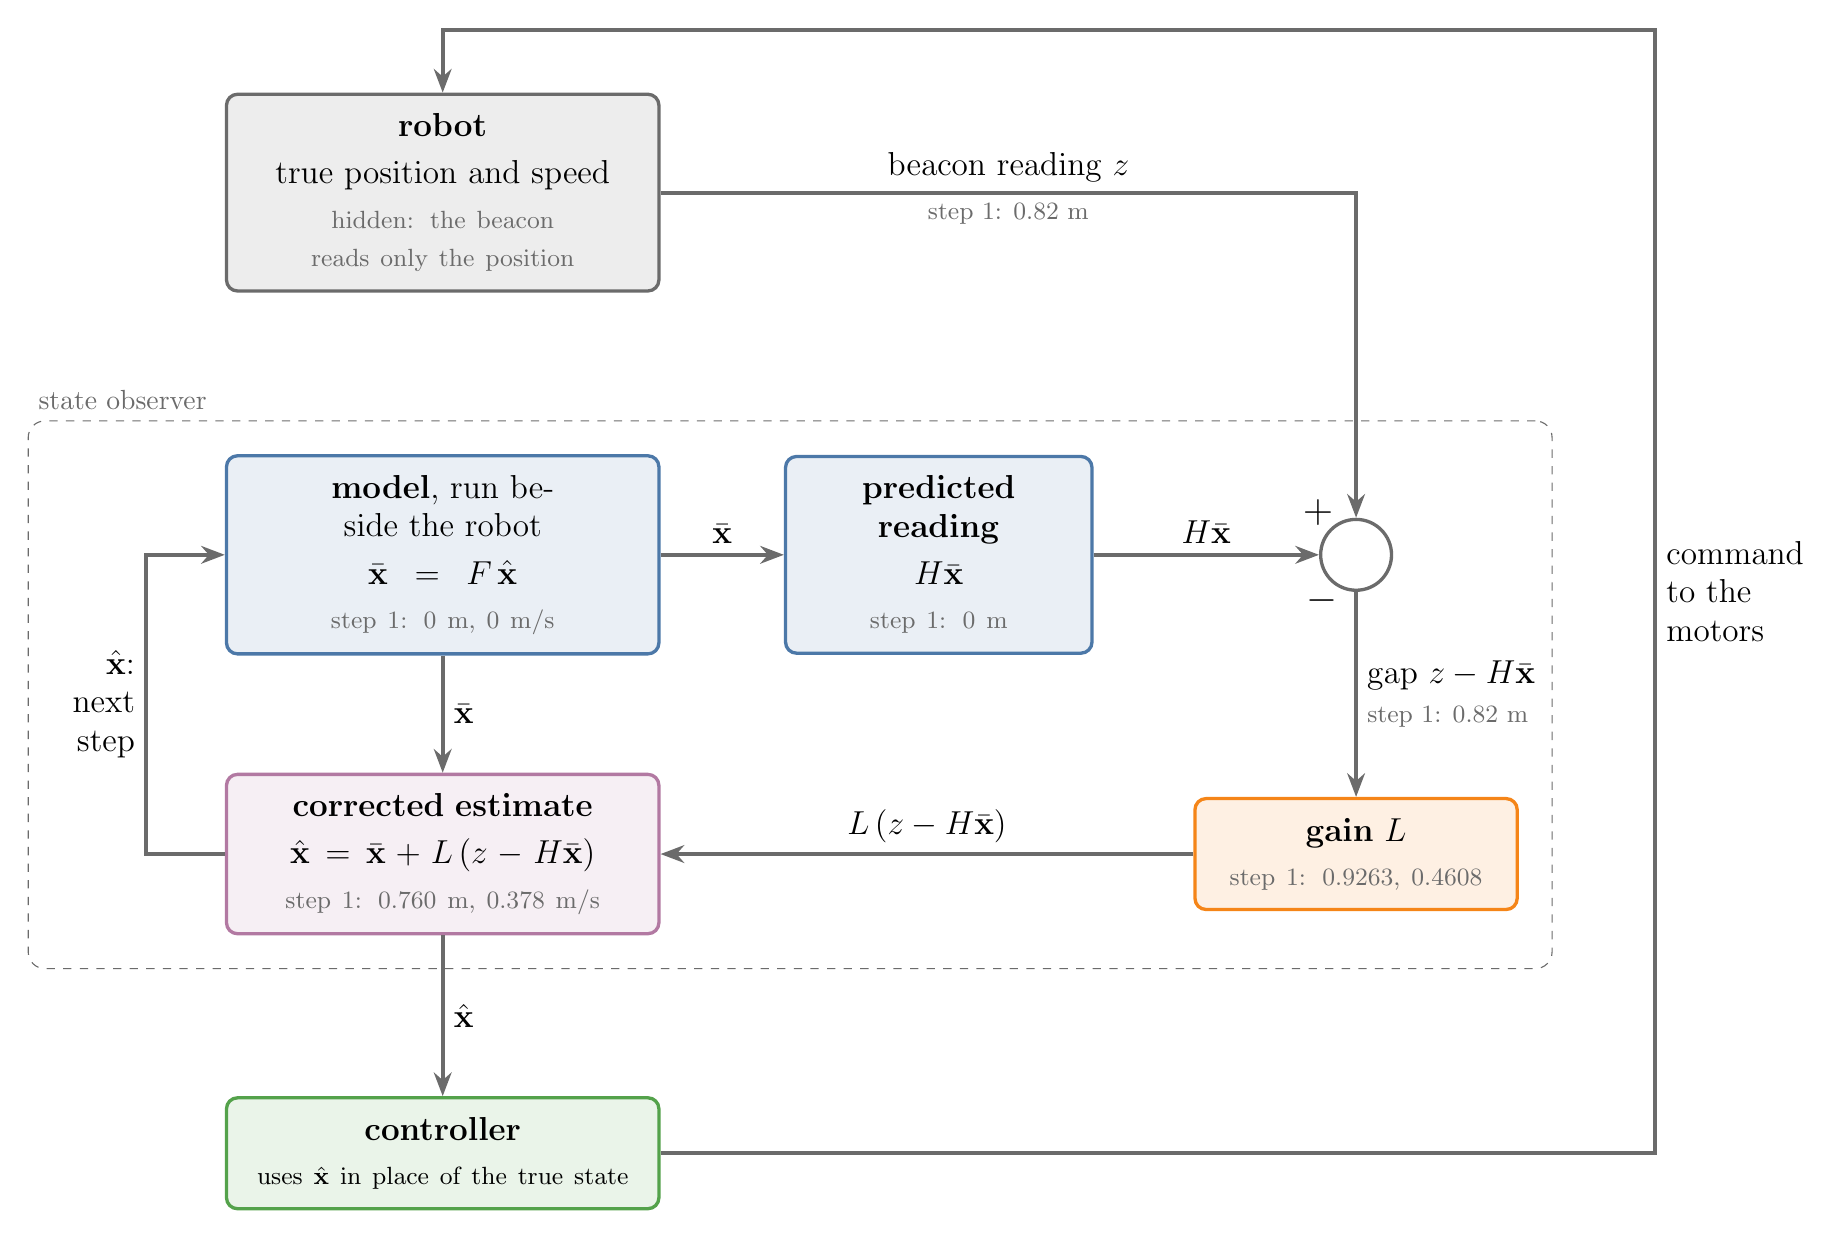
\begin{tikzpicture}[every node/.append style={font=\large}]
  \node[box=cgrey, text width=5cm] (robot) at (0,4.6) {\textbf{robot}\\[3pt] true position and speed\\[2pt]
     \small\textcolor{cgrey}{hidden: the beacon reads only the position}};
  \node[box=cblue, text width=5cm] (model) at (0,0) {\textbf{model}, run beside the robot\\[3pt]
     $\bar{\mathbf{x}} = F\,\hat{\mathbf{x}}$\\[2pt] \small\textcolor{cgrey}{step 1: 0 m, 0 m/s}};
  \node[box=cblue, text width=3.4cm] (pred) at (6.3,0) {\textbf{predicted reading}\\[3pt] $H\bar{\mathbf{x}}$\\[2pt]
     \small\textcolor{cgrey}{step 1: 0 m}};
  \node[circle, draw=cgrey, fill=white, minimum size=0.9cm, inner sep=0pt] (cmp) at (11.6,0) {};
  \node[font=\Large] at ($(cmp.north west)+(-0.15,0.2)$) {$+$};
  \node[font=\Large] at ($(cmp.south west)+(-0.1,-0.25)$) {$-$};
  \node[box=corange, text width=3.6cm] (gain) at (11.6,-3.8) {\textbf{gain} $L$\\[2pt]
     \small\textcolor{cgrey}{step 1: 0.9263, 0.4608}};
  \node[box=cpurple, text width=5cm] (est) at (0,-3.8) {\textbf{corrected estimate}\\[3pt]
     $\hat{\mathbf{x}} = \bar{\mathbf{x}} + L\,(z - H\bar{\mathbf{x}})$\\[2pt]
     \small\textcolor{cgrey}{step 1: 0.760 m, 0.378 m/s}};
  \node[box=cgreen, text width=5cm] (ctrl) at (0,-7.6) {\textbf{controller}\\[2pt]
     \small uses $\hat{\mathbf{x}}$ in place of the true state};
  % the real reading and the predicted reading meet at the comparison
  \draw[arrow] (robot.east) -- node[above] {beacon reading $z$}
     node[below, font=\small, text=cgrey] {step 1: 0.82 m} (11.6,4.6) -- (cmp.north);
  \draw[arrow] (model.east) -- node[above] {$\bar{\mathbf{x}}$} (pred.west);
  \draw[arrow] (pred.east) -- node[above] {$H\bar{\mathbf{x}}$} (cmp.west);
  \draw[arrow] (cmp.south) -- node[right, align=left] {gap $z - H\bar{\mathbf{x}}$\\
     \small\textcolor{cgrey}{step 1: 0.82 m}} (gain.north);
  % the gap times the gain corrects the model's estimate
  \draw[arrow] (gain.west) -- node[above] {$L\,(z - H\bar{\mathbf{x}})$} (est.east);
  \draw[arrow] (model.south) -- node[right] {$\bar{\mathbf{x}}$} (est.north);
  % the estimate goes back into the model for the next step, and on to the controller
  \draw[arrow] (est.west) -- ++(-1.0,0) |- node[pos=0.25, left, align=right] (nxt) {$\hat{\mathbf{x}}$:\\ next\\ step}
     (model.west);
  \draw[arrow] (est.south) -- node[right] {$\hat{\mathbf{x}}$} (ctrl.north);
  \draw[arrow] (ctrl.east) -- (15.4,-7.6) |- node[pos=0.25, right, align=left] {command\\ to the\\ motors}
     ($(robot.north)+(0,0.8)$) -- (robot.north);
  % the observer: everything that runs in the robot's computer between the sensor and the controller
  \coordinate (loop) at ($(est.west)+(-1.0,0)$);
  \begin{scope}[on background layer]
    \node[draw=cgrey, dashed, rounded corners=6pt, inner sep=12pt, fit=(model) (pred) (cmp) (gain) (est) (loop) (nxt)]
          (obs) {};
  \end{scope}
  \node[note, font=\normalsize, anchor=south west] at (obs.north west) {state observer};
\end{tikzpicture}
\end{document}
